% "Станет проще"

\documentclass[a4paper,12pt]{article} % тип документа

% report, book

%  Русский язык

\usepackage[T2A]{fontenc}			% кодировка
\usepackage[utf8]{inputenc}			% кодировка исходного текста
\usepackage{graphicx}
\usepackage[english,russian]{babel}	% локализация и переносы



\usepackage[left=20mm, top=10mm, right=20mm, bottom=10mm, nohead, nofoot]{geometry}
% Математика
\usepackage{amsmath,amsfonts,amssymb,amsthm,mathtools} 
\usepackage{csvsimple}
\usepackage{multirow}


\usepackage{wasysym}
\usepackage{subcaption}
\usepackage{gensymb}
\usepackage{verbatim}
\usepackage[hidelinks]{hyperref}
\usepackage{float}
\usepackage{enumerate}
\usepackage{wrapfig}
\usepackage{listings} %написание кода
%\usepackage{fancyhdr}

\usepackage[dvipsnames]{xcolor}
\usepackage{verbatim} %comments

%Заговолок



\graphicspath{ {img/} }





\begin{document}


\thispagestyle{empty}


\includegraphics[width=4cm]{logo.png}\\

\section{Вентили}

\begin{table}[H]
\begin{tabular}{|l|l|l|l|l|l|l|l|l|l|l|}
\cline{1-3} \cline{5-7} \cline{9-11}
\multicolumn{3}{|l|}{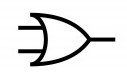
\includegraphics[width=1.1cm]{or.jpg}} &  & \multicolumn{3}{l|}{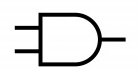
\includegraphics[width=1.1cm]{and.jpg}}  &  & \multicolumn{3}{l|}{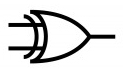
\includegraphics[width=1.1cm]{xor.jpg}}  \\ \cline{1-3} \cline{5-7} \cline{9-11} 
$ A  $      & $B$      &$ A+B $     &  &$ A  $    & $B$      & $A \times B$     &  &$ A  $       & $B$      & $A \oplus B$     \\ \cline{1-3} \cline{5-7} \cline{9-11} 
1      & 0      & 1        &  & 1      & 0      & 0       &  & 1      & 0      & 1       \\ \cline{1-3} \cline{5-7} \cline{9-11} 
0      & 1      & 1        &  & 0      & 1      & 0       &  & 0      & 1      & 1       \\ \cline{1-3} \cline{5-7} \cline{9-11} 
0      & 0      & 0        &  & 0      & 0      & 0       &  & 0      & 0      & 0       \\ \cline{1-3} \cline{5-7} \cline{9-11} 
1      & 1      & 1        &  & 1      & 1      & 1       &  & 1      & 1      & 0       \\ \cline{1-3} \cline{5-7} \cline{9-11} 
\end{tabular}
\end{table}
\large{
Двоичное исчисление:\\
$1_2 + 1_2 = 10_2 $\\
$1111_2 = 2^3 + 2^2 + 2^1 + 26 $




\begin{minipage}{0.45\textwidth}

\begin{center}


 \Large { CD4073BE}

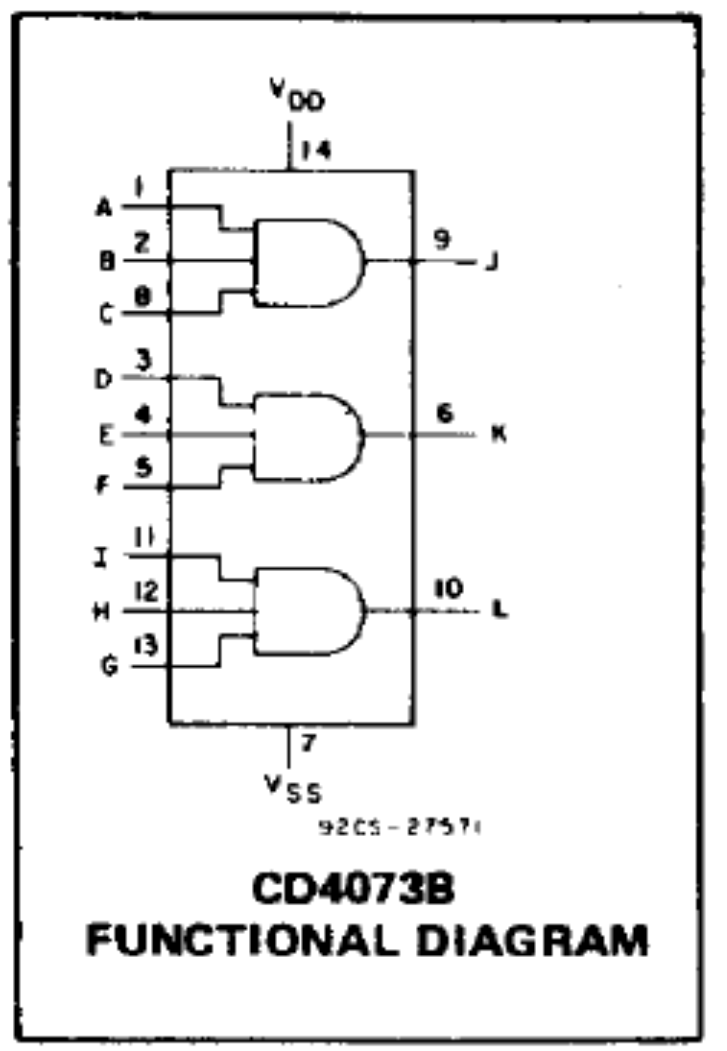
\includegraphics[width=5cm]{and.png}\\
\end{center}
\end{minipage}%
\hfill
\begin{minipage}{0.45\textwidth}
\begin{tabular}{|p{\textwidth}}

\begin{center}
 \LARGE {SN74HC86N}
\end{center}
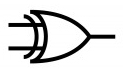
\includegraphics[width=6cm]{xor.png}
\begin{center}
\LARGE{$Y = A \oplus B $} \\
\vspace{0.5cm}

\end{center}

 
\end{tabular}
\end{minipage}%




















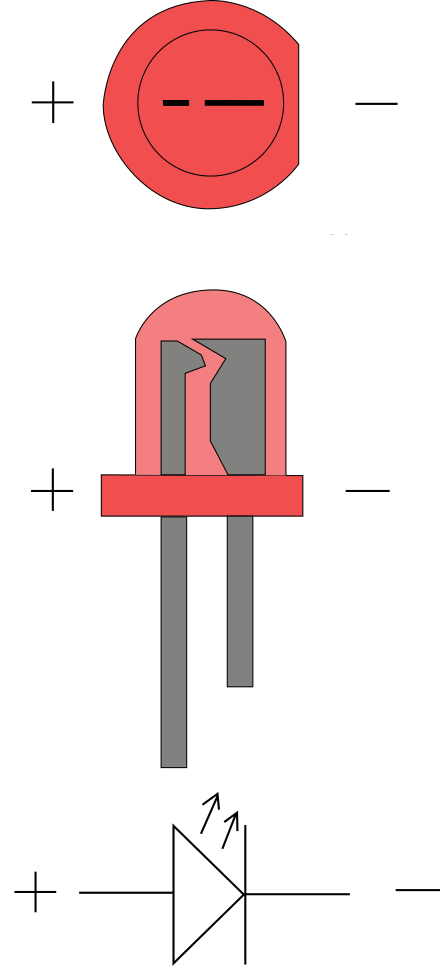
\includegraphics[width=3cm]{diode.png}





\end{document}
